\documentclass[12pt]{article}
\usepackage{float}
% Packages for formatting
\usepackage{graphicx}    % For including images
\usepackage{fancyhdr}    % For custom headers and footers
\usepackage{geometry}    % For setting page margins
\usepackage{amsmath}     % For advanced mathematical formatting
\usepackage{hyperref}    % For hyperlinks

% Page margins
\geometry{
    a4paper,
    left=1in,
    right=1in,
    top=1in,
    bottom=1in
}

% Header and Footer settings
\pagestyle{fancy}
\fancyhf{} % Clear all header and footer fields
\fancyhead[L]{\textbf{OS LAB TASK 7}}         % Left header
\fancyhead[R]{\textbf{FAST NUCES}}     % Right header
\fancyfoot[C]{\thepage}                % Center footer with page number

% Title Information
\title{
    \vspace{-2cm} % Adjust vertical spacing
    \LARGE{\textbf{Operating Systems Lab Report}} \\
    \vspace{0.5cm}
    \Huge{Muhammad Shafeen} \\
    \Large{Student ID: 22P-9278}
}
\date{} % No date

\begin{document}

\maketitle
\thispagestyle{fancy} % Apply the fancy header to the title page

\section*{Lab 7: Operating Systems}

\section{Exercise 2 :}
\subsection{Question : }
Model a fork() call in C/C++ so that your pro-
gram can create a total of EXACTLY 6 pro-
cesses (including the parent). (Note: You may
check the number of processes created using
the method from Exercise 1 (Section-3.2.1.1 by
using a sleep of 60 seconds or more and enter-
ing eithe ps, or pstree in another terminal).
\subsection{Answer :}
\begin{figure}[H]
    \centering
    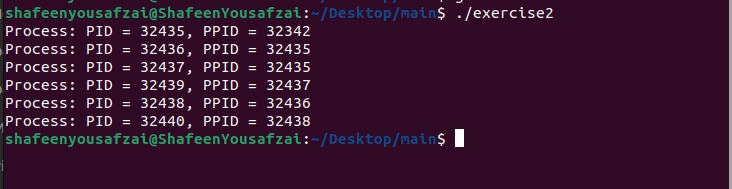
\includegraphics[width=\textwidth]{12313.png}
    \caption{This is the output for 1 parent and 5 child processes , total 6}
    \label{fig:enter-label}
\end{figure}

\section{Running States}

\subsection*{Code}

% Placeholder for code image
\begin{figure}[h]
    \centering
    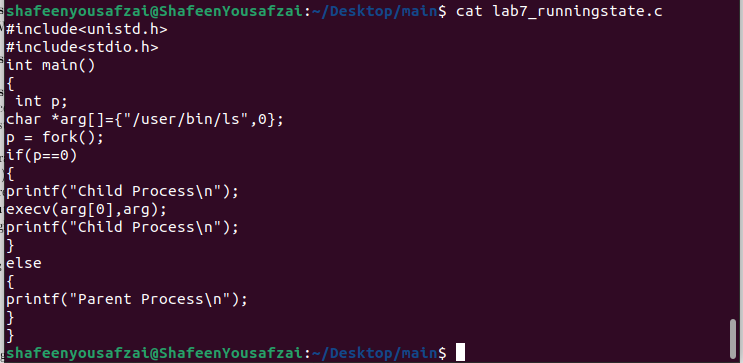
\includegraphics[width=\textwidth]{Screenshot from 2024-10-04 04-14-27.png} % Replace with your image path
    \caption{Code for Running States}
    \label{fig:running_states_code}
\end{figure}

\begin{figure}[H]
    \centering
    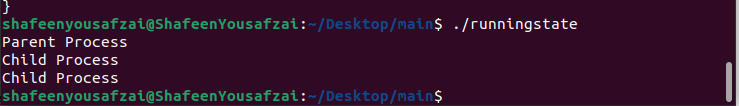
\includegraphics[width=\textwidth]{Screenshot from 2024-10-04 04-14-38.png} % Replace with your image path
    \caption{Output of the code}
    \label{fig:waiting_states_solution}
\end{figure}

\subsection*{Questions and Answers}

\textbf{Q1: What is the first argument to the \texttt{execv()} call? What is its content?}

\textbf{Answer:} The first argument to the \texttt{execv()} function is the path to the executable file that you want to run. In our case, the path is \texttt{"/bin/ls"}, which specifies the \texttt{ls} command to list directory contents.

\bigskip

\textbf{Q2: What is the second argument to it? What is its content?}

\textbf{Answer:} The second argument is an array of argument strings (\texttt{argv}) passed to the executable. This array must be terminated with a NULL pointer. It typically starts with the name of the executable itself, followed by any additional arguments. For example, \texttt{argv[0]} is the program name, and \texttt{argv[1]} onwards are the arguments.

\bigskip

\textbf{Q3: What is \texttt{arg}?}

\textbf{Answer:} \texttt{arg} is the array that contains the command-line arguments and the path to the executable that you want to run. It is used by \texttt{execv()} to replace the current process image with a new process image. The array is terminated with a NULL pointer to indicate the end of arguments.

\bigskip

\textbf{Q4: Look at the code of the child process (\texttt{p == 0}). How many times does the statement “Child Process” appear? Why?}

\textbf{Answer:} The statement “Child Process” appears only once because after the \texttt{execv()} call is executed, the child process is replaced by the new executable. Therefore, the original code (including any further print statements) does not continue to execute in the child process.

\section{Waiting States Exercise - 3.2.3.1 Sleep()}

\subsection*{Problem}

Write a C program that can display a count from 10 to 0 (in reverse order) using a \texttt{for} or a \texttt{while} loop. Each number should be displayed after a delay of 1 second.

\subsection*{Solution}

% Placeholder for solution image or code


\begin{figure}[H]
    \centering
    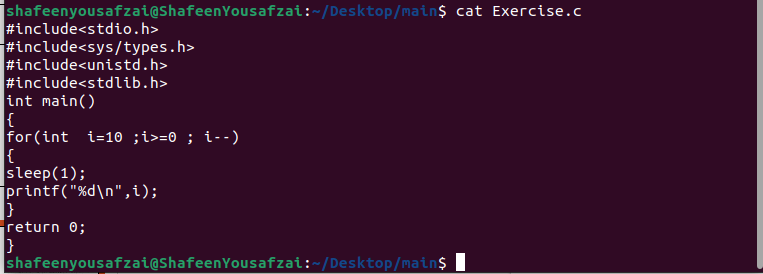
\includegraphics[width=\textwidth]{1.png} % Replace with your image path
    \caption{C Program Solution for Waiting States Exercise}
    \label{fig:waiting_states_solution}
\end{figure}

\bigskip

Below is the C program that accomplishes the task:

\begin{verbatim}
#include<stdio.h>
#include<sys/types.h>
#include<unistd.h>
#include<stdlib.h>
int main() 
{
for(int  i=10 ;i>=0 ; i--)
{
sleep(1);
printf("%d\n",i);
}
return 0;
}
\end{verbatim}

\section{Exit() Call}
\begin{figure}[H]
    \centering
    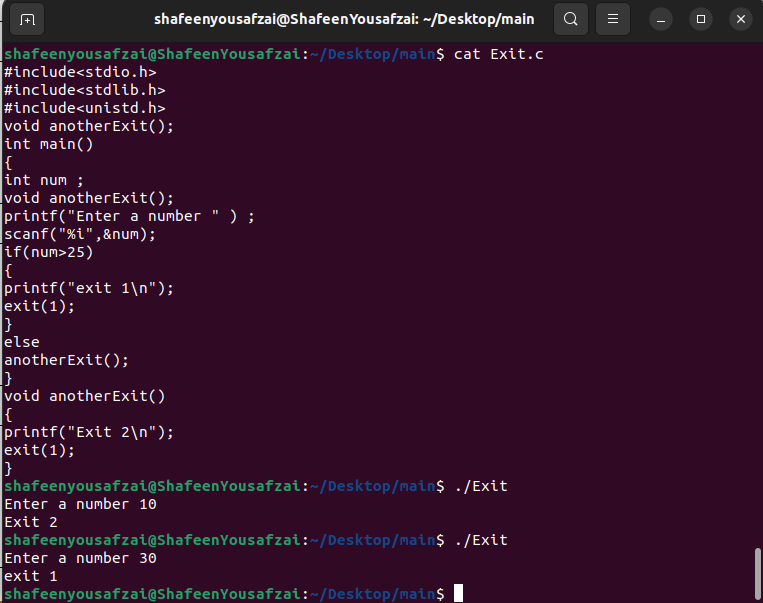
\includegraphics[width=0.8\linewidth]{image1.png}
    \caption{Caption}
    \label{fig:enter-label}
\end{figure}

\begin{verbatim}
#include<stdio.h>
#include<stdlib.h>
#include<unistd.h>
void anotherExit();
int main()
{
int num ;
void anotherExit();
printf("Enter a number " ) ;
scanf("%i",&num);
if(num>25)
{
printf("exit 1\n");
exit(1);
}
else
anotherExit();
}
void anotherExit()
{
printf("Exit 2\n");
exit(1);
}
\end{verbatim}

\subsection*{Question}

Can you identify which \texttt{exit()} call is being used each time a program exits?

\subsection*{Answer}

Yes, the \texttt{exit()} function is called with different status codes based on the input:

\begin{itemize}
    \item When entering a number below 25, \texttt{exit(2)} is called.
    \item When entering a number above 25, \texttt{exit(1)} is called.
\end{itemize}

These exit codes can be used to indicate different termination reasons to the operating system or calling processes.

\section{Atexit() Call}

% Placeholder for atexit() call image or code
\subsection{Code : }
\begin{figure}[H]
    \centering
    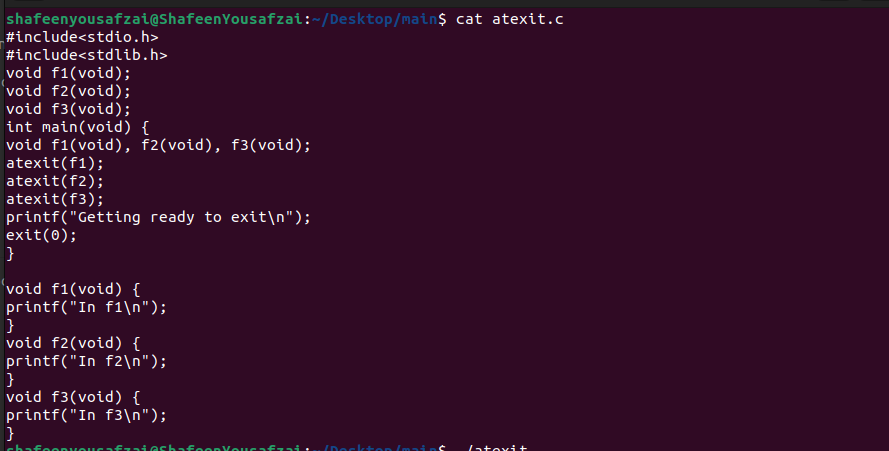
\includegraphics[width=\textwidth]{2.png}
    \caption{Caption}
    \label{fig:enter-label}
\end{figure}

\subsection{Execution of Code : }
\begin{figure}[H]
    \centering
    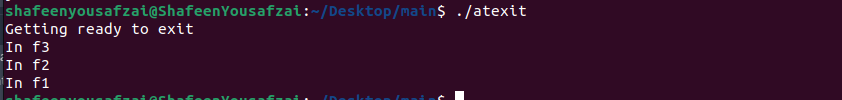
\includegraphics[width=\textwidth]{3.png}
    \caption{Output of the above code}
    \label{fig:enter-label}
\end{figure}



\subsection*{Explanation}

The \texttt{atexit()} function allows you to register functions to be called upon normal program termination. This can be useful for performing cleanup tasks such as freeing allocated memory, closing files, or other housekeeping activities.

\bigskip

\textbf{Example Usage:}

\begin{verbatim}
#include<stdio.h>
#include<stdlib.h>
void f1(void);
void f2(void);
void f3(void);
int main(void) {
void f1(void), f2(void), f3(void);
atexit(f1);
atexit(f2);
atexit(f3);
printf("Getting ready to exit\n");
exit(0);
}

void f1(void) {
printf("In f1\n");
}
void f2(void) {
printf("In f2\n");
}
void f3(void) {
printf("In f3\n");
}
\end{verbatim}

In this example, the \texttt{cleanup} function is registered to be called when the program exits normally.

\subsection{Question 1 : }
What is the difference between exit() and
atexit()? What do they do? (Check man
atexit and man 3 exit ).
\subsection{Answer 1: }
\begin{figure}[H]
    \centering
    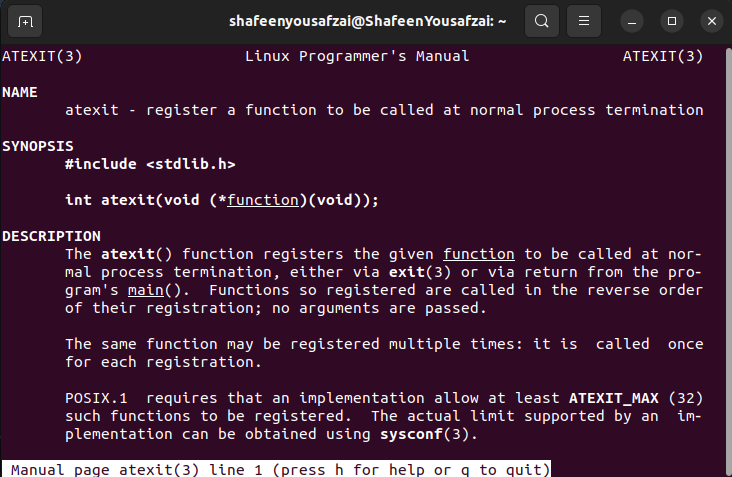
\includegraphics[width=\textwidth]{4.png}
    \caption{This is the man for atexit()}
    \label{fig:enter-label}
\end{figure}

\begin{figure}[H]
    \centering
    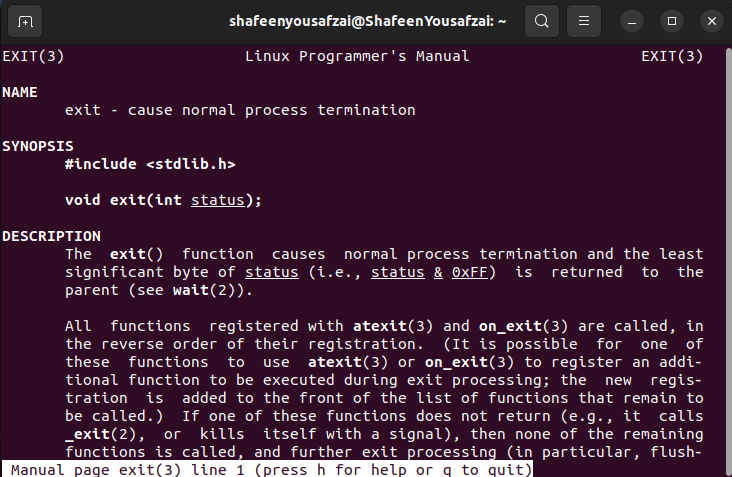
\includegraphics[width=\textwidth]{12.png}
    \caption{This is the man for exit()}
    \label{fig:enter-label}
\end{figure}


\textbf{exit()}: Terminates the program execution.\\
behaviour:  \\
        Performs cleanup such as flushing standard I/O buffers.
        Calls all functions registered with atexit() in the reverse order of their registration.
        Returns control to the host environment with the specified exit status.\\
\textbf{atexit()} : Registers functions to be automatically called upon normal program termination.\\
behaviour: \\
\hfill(1em)        Allows multiple functions to be registered.
        Registered functions are executed in the reverse order of their registration when exit() is called.
        Useful for cleanup tasks like freeing resources or saving state.


\subsection{Question 2 :}
What does the 0 provided in the exit() call
mean? What will happen if we change it
to 1? (Check manual page for exit)
\subsection{Answer 2 :}
The 0 in exit(0) indicates successful program termination. Changing it to 1 signals an error or abnormal termination.
\subsection{Question 3 :}
Q2 ) What does the 0 provided in the exit() call
mean? What will happen if we change it
to 1? (Check manual page for exit)
\subsection{Answer 3 : }
If `exit()` is called in `f1`, `f2`, or `f3`, the program will terminate immediately, and any remaining `atexit()`-registered functions will not be executed.
\subsection{Question 4 :}
Why do you think we are getting reverse
order of execution of atexit calls?
\subsection{Answer 4 : }
The `atexit()` functions are executed in reverse order of registration to ensure proper cleanup, similar to how stack unwinding works. This way, the most recently registered function is called first, ensuring that resources are released in the correct sequence.

\section{3.2.4.3 Abort Call}
\subsection{Question 1 :}
Q1 Check the man pages for abort. How
does the abort call terminate the pro-gram? What is the name of the particular signal?
\subsection{Answer 1 :}
\begin{figure}[H]
    \centering
    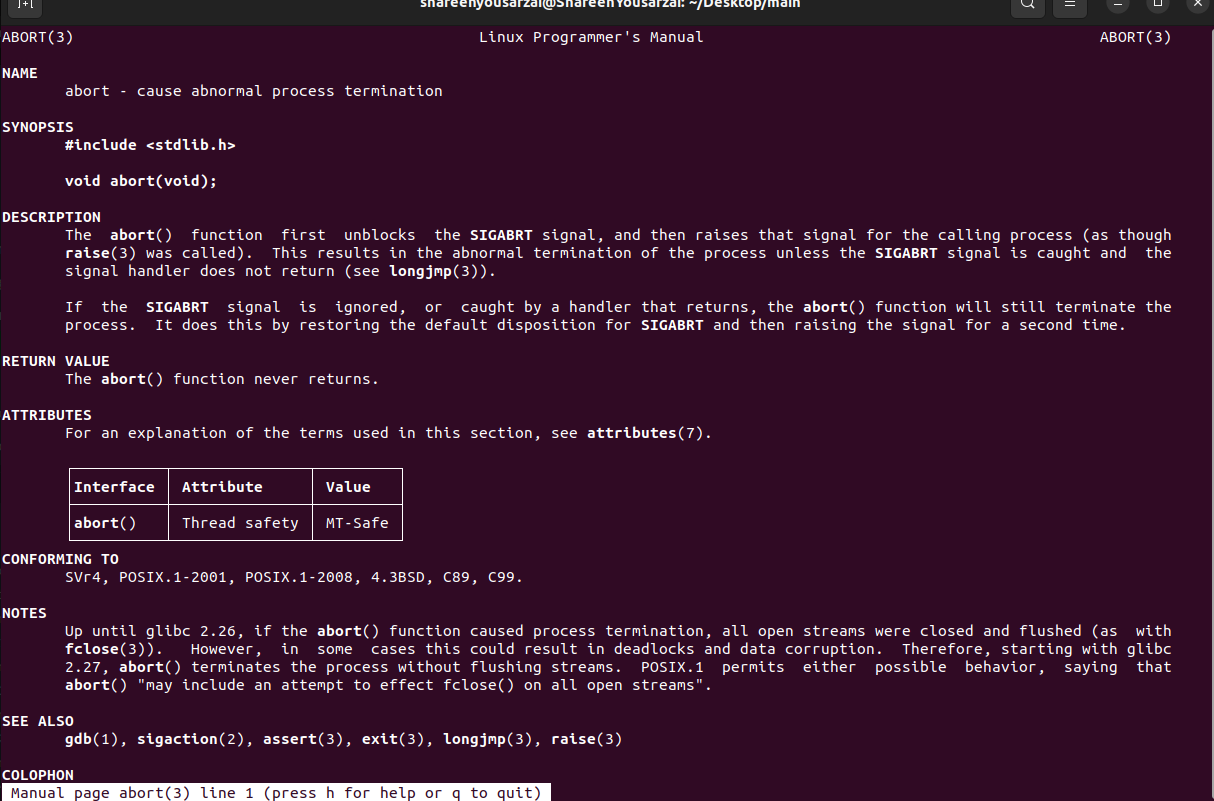
\includegraphics[width=\textwidth]{asdasd.png}
    \caption{This is the screenshot of man abort}
    \label{fig:enter-label}
\end{figure}
The `abort()` call terminates the program by generating the \textbf{SIGABRT}* signal, which causes an abnormal program termination. This signal is used to indicate a serious program error and usually results in a core dump for debugging purposes.
\subsection{Question 2 :}
Q2 Execute your program. What is the out-
put of our program?
\subsection{Answer 2 :}
\begin{figure}[H]
    \centering
    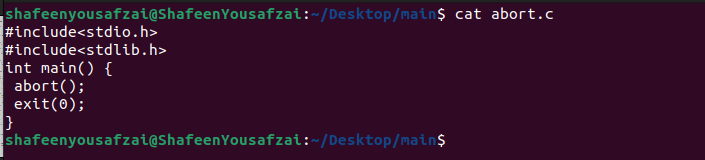
\includegraphics[width=\textwidth]{111.png}
    \caption{Runnig the code and checking its output}
    \label{fig:enter-label}
\end{figure}

\begin{figure}[H]
    \centering
    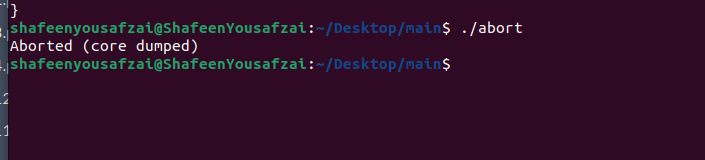
\includegraphics[width=\textwidth]{21312.png}
    \caption{output of the running code}
    \label{fig:enter-label}
\end{figure}

The program terminates immediately with an abnormal termination due to the abort() call, so exit(0) is not reached, and no output is produced.


\subsection{Question 3 :}
Q3 Include the abort call in function f3 in our
code provided for Atexit() call. How does
our program terminate using this?
\subsection{Answer 3 :}

\begin{figure}[H]
    \centering
    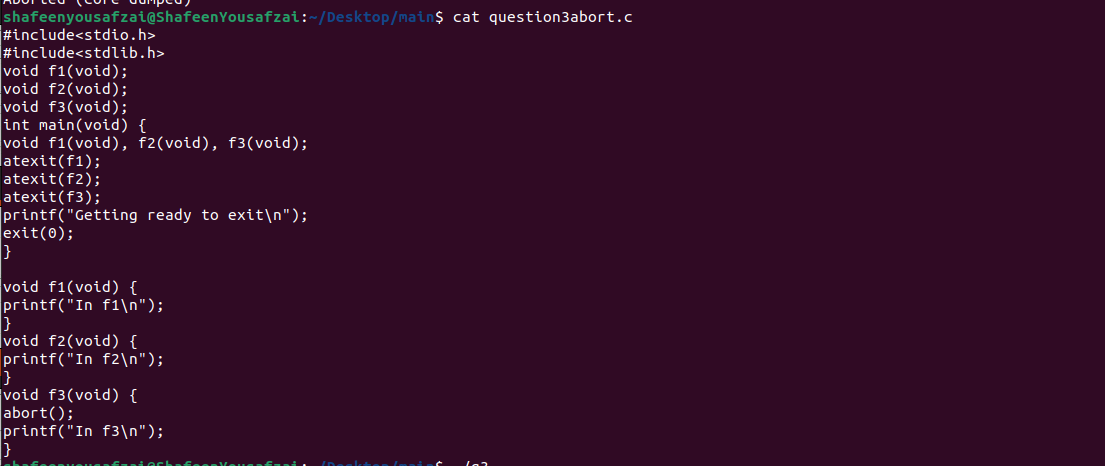
\includegraphics[width=\textwidth]{sada.png}
    \caption{Showing the code with abort}
    \label{fig:enter-label}
\end{figure}

\begin{figure}[H]
    \centering
    
\includegraphics[width=\textwidth]{eqew.png}
    \caption{Executing code}
    \label{fig:enter-label}
\end{figure}

If abort() is called in f3, the program terminates immediately with a SIGABRT signal, preventing any further execution of remaining atexit() functions.

\section{3.2.4.4 Kill Call}
KILL -l
9)th    
SIGKILL is a signal in Unix-like operating systems that is used to immediately terminate a process. It has the following characteristics

\begin{figure}[H]
    \centering
    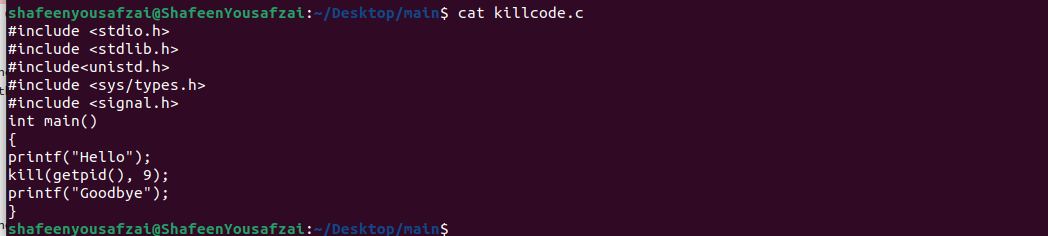
\includegraphics[width=\textwidth]{asdqw.png}
    \caption{The kill code , Showing the code}
    \label{fig:enter-label}
\end{figure}

\begin{figure}[H]
    \centering
    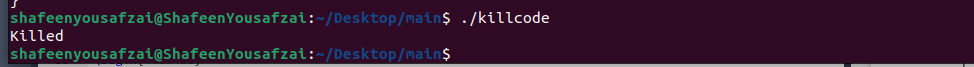
\includegraphics[width=\textwidth]{21321.png}
    \caption{This is the demonstration code provided in manual }
    \label{fig:enter-label}
\end{figure}

\subsection{Question Code : }
\begin{figure}[H]
    \centering
    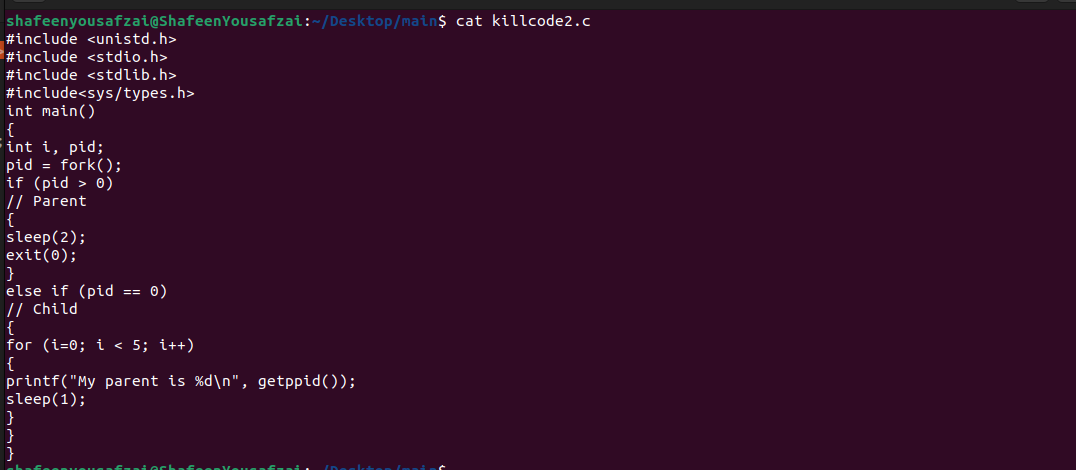
\includegraphics[width=\textwidth]{1212.png}
    \caption{This is the Questions code}
    \label{fig:enter-label}
\end{figure}

\begin{figure}[H]
    \centering
    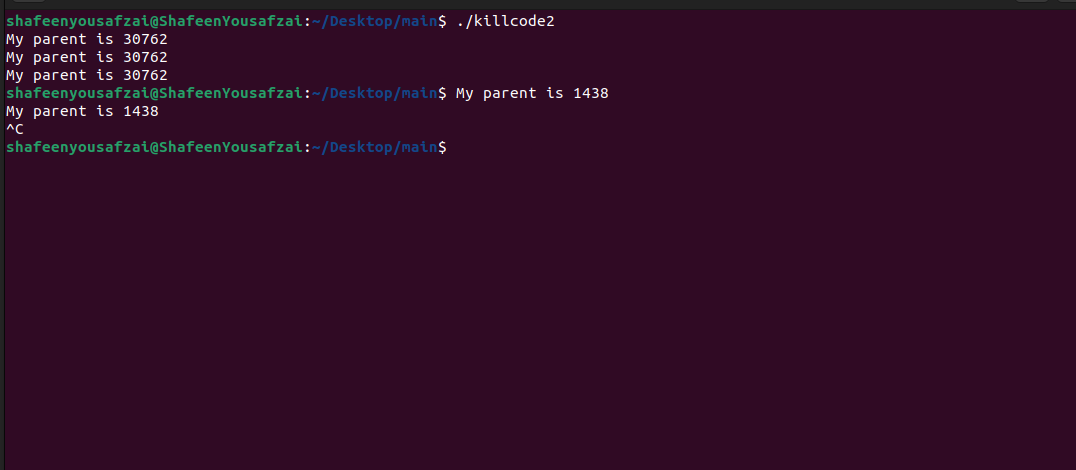
\includegraphics[width=\textwidth]{sadsa.png}
    \caption{Exection of the code}
    \label{fig:enter-label}
\end{figure}

\subsection{Question 1:}
What are the PPID values you are receiv-ing from the for loop?
\subsection{Answer 1:}
The PPID values received from the loop are: 
   38762,38762,38762,1438,1438
 

\subsection{Question 2 :}
What has happened when the numbers of the PPID change?
\subsection{Answer 2: }
After two seconds (when the parent process calls exit(0)), the child becomes an orphan. The init process (typically PID 1) adopts the child, so the PPID changes to the PID of the init process.
\subsection{Question 3 :}
What is now PID of the init process?
\subsection{Answer 3 :}
The PID of the init process is typically 1. Once the parent process exits, the child process's PPID changes to 1, indicating that it has been adopted by the init process.
The word mentioned next to signal 9 (`kill -l`) is: SIGKILL
\begin{itemize}
    \item [Answer:]
    % Insert your answer here
\end{itemize}

\section{3.3.1 Parent Dies Before Child}
\begin{figure}[H]
        \centering
        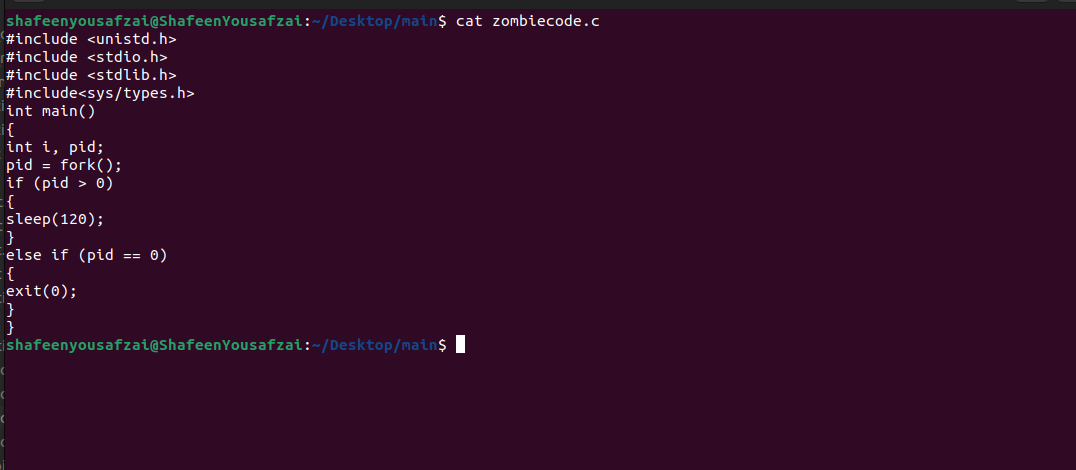
\includegraphics[width=\textwidth]{sadsada.png}
        \caption{Original Code for analysis}
        \label{fig:enter-label}
    \end{figure}
    % Insert your answer here

\subsection{Exection of code}
\begin{figure}[H]
    \centering
    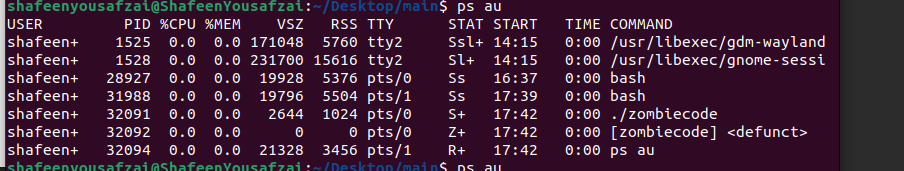
\includegraphics[width=\textwidth]{3213.png}
    \caption{This is the part before sleep happens}
    \label{fig:enter-label}
\end{figure}
\subsection{Both child and parent \\processes have been killed}
\begin{figure}[H]
    \centering
    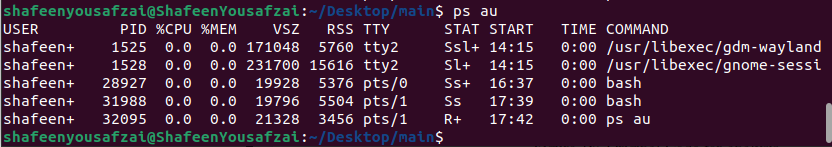
\includegraphics[width=\textwidth]{dsadsada.png}
    \caption{This is the part after sleep happens}
    \label{fig:enter-label}
\end{figure}

\end{document}
